%%%%%%%%%%%%%%%%%%%%%%% file template.tex %%%%%%%%%%%%%%%%%%%%%%%%%
%
% This is a general template file for the LaTeX package SVJour3
% for Springer journals.          Springer Heidelberg 2006/03/15
%
% Copy it to a new file with a new name and use it as the basis
% for your article. Delete % signs as needed.
%
% This template includes a few options for different layouts and
% content for various journals. Please consult a previous issue of
% your journal as needed.
%
%
% 5th Mar 2012
% NOTES for MISTA 2013
% This template has been supplied for use for the MISTA 2013 conference
% In essence it is the same as the one supplied by SV, but with additional comments
% The reason this template is being used is to make it as easy as possible
% to be able to submit to the post conference special issue of the Journal
% of Scheduling
%%%%%%%%%%%%%%%%%%%%%%%%%%%%%%%%%%%%%%%%%%%%%%%%%%%%%%%%%%%%%%%%%%%
%

% For MISTA 2013, use the default option that has been supplied
\documentclass{svjour3}                     % onecolumn (standard format)
%\documentclass[smallextended]{svjour3}     % onecolumn (second format)
%\documentclass[twocolumn]{svjour3}         % twocolumn

\smartqed  % flush right qed marks, e.g. at end of proof

\usepackage{graphicx}
\DeclareGraphicsExtensions{.eps}
\graphicspath{{figures/}}

\usepackage{mathptmx}      % use Times fonts if available on your TeX system
%
% insert here the call for the packages your document requires
\usepackage{latexsym}
\usepackage{amsmath,amssymb}

% please place your own definitions here and don't use \def but
% \newcommand{}{}
\include{shorthand} % put your own shorthand declarations in this document
\usepackage{rotating}

% Insert the name of "your journal" with
% This is preset for MISTA 2013: Do not change
\journalname{MISTA 2013}
%
\begin{document}

\title{Generating Training Data for Learning Linear Composite Dispatching Rules for Scheduling}

%\subtitle{Do you have a subtitle?\\ If so, write it here}

\author{Helga Ingimundardottir \and Thomas Philip Runarsson 
}

\institute{Helga Ingimundardottir \at
              University of Iceland \\
              \email{hei2@hi.is}           %  \\
           \and
           Thomas Philip Runarsson \at
              University of Iceland \\
              \email{tpr@hi.is}           %  \\
}

\maketitle

\begin{abstract}
A supervised learning approach to generating composite linear priority dispatching rules for scheduling is studied. In particular we investigate a number of strategies for generating training data for learning a linear dispatching rule using preference learning. The results show that generating training data set from optimal solutions only is not as effective as when suboptimal solutions are added to the set. Furthermore, different strategies for creating preference pairs is investigated as well as sub-optimal solution trajectories. The different strategies are investigated on 2000 randomly generated problem instances using two different problems generator settings.
\end{abstract}
\section{Introduction}
The job-shop scheduling problem (JSP) deals with the allocation of tasks of competing resources where the goal is to optimise a single or multiple objectives, in particular minimising a schedule's maximum completion time, i.e. the makespan. Due to difficulty in solving this problem heuristics are common applied. Perhaps the simplest approach to generating good solutions to the JSP is by applying dispatching rules \cite{Panwalkar77}. For example, dispatching a job which has the most work remaining (MWR). Composites of such simple rules can perform significantly better 
\cite{Jayamohan04}. As a consequence a linear composite of dispatching rule was presented by the authors in 
\cite{InRu11a}. There the goal was to learn a set of weights, $\vec{w}$ via logistic regression such that 
\begin{equation}\label{eq:jssp:linweights}
h(\vec{x}_j)=\inner{\vec{w}}{\vphi(\vec{x}_j)},
\end{equation}
yields the preference estimate for dispatching the job $j$ that corresponds to post-decision state $\vec{x}_j$, where $\vphi(\vec{x}_j)$ denotes the feature mapping. 
The features may correspond to a dispatching rule, for example if only the single feature $\phi_6(\vec{x}_j) $ is applied it would correspond to MWR heuristic, namely yielding $h(\vec{x}_j)>h(\vec{x}_i)$, $\forall i$ which are jobs with less work remaining than job $j$. 

The weights in \cite{InRu11a} then found using supervised learning, where the training data was created from optimal solutions of randomly generated problem instances. As an alternative would be to minimizing the mean makespan directly using a brute force search such as the CMA-ES \cite{Hansen01}. This actually results in a better linear composite priority dispatching rules. The nature of the CMA-ES search is to explore suboptimal routes until it converges to an optimal one. Implying that the previous approach of only looking into one optimal route may not produce a sufficient rich training set. That is, the training set should incorporate a more complete knowledge on \emph{all} possible preferences, i.e. make also the distinction between suboptimal and sub-suboptimal features, etc.  This would require a Pareto ranking of preferences which can be used to make the distinction to which feature sets are equivalent, better or worse -- and to what degree, i.e. by giving a weight to the preference. This would results in a very large training set, which of course could be re-sampled in order to make it computationally feasible to learn. Here we will investigate a number of different ranking strategies for creating preference pairs.

Alternatively, training data could be generated using sub-optimal solution trajectories. For instance~\cite{Siggi05} used decision trees to `rediscover' the largest processing time (LPT) single priority based dispatching rule by 
using the dispatching rule to create its training data. The limitations of using heuristics to label the training data is that the learning algorithm will mimic the original heuristic (both when it works poorly and well on the problem instances) and does not consider the real optimum. In order to learn heuristics that can outperform existing heuristics, then the training data needs to be correctly labelled. This drawback is confronted in~\cite{Malik08,Russell09,Siggi10} by using an optimal scheduler, computed off-line. Here we will both follow optimal and sub-optimal solution trajectories, but for each partial solution the preference pair will be labelled correctly by solving the partial solution to optimality using a commercial software package \cite{gurobi}. For this study only MWR, the promising single priority dispatching rule (see~\cite{InRu12a}) for the given data distributions, and the CMA-ES found linear dispatching rule will be deemed worthwhile for generating suboptimal trajectories.

In summary, the paper considers two main aspects of the generation of the training data, 
\begin{enumerate}
\item how preference pair are created at each decision stage, and
\item which solution trajectorie(s) should be sampled. That is, optimal, random, sub-optimal based on a good 
heuristic, etc.
\end{enumerate}

The paper first illustrates how the JSP problem can be seen as a decision tree where the depth of the tree corresponds 
to the number of job dispatches needed to form a complete schedule. The feature space is also introduced and how 
optimal dispatches and sub-optimal dispatches are labelled as each node in the tree. This is followed by a section 
detailing the strategies investigated in this paper for selecting preference pairs ranking and sampling solution 
trajectories. We then perform an extensive study comparing these strategies, followed by a conclusion and summary of 
main results.

\begin{table}  
  \caption{Feature space $\mathcal{F}$ for JSP where job $J_j$ on machine $M_a$ given the resulting temporal schedule after dispatching $(j,a)$.  }
  \label{tbl:jssp:feat}
  \input{tables/features-description-nomath}
\end{table}

\section{JSP tree representation}\label{sec:gen:gametree}
When building a complete JSP schedule $\ell=n\cdot m$ ($n$ jobs and $m$ machines) dispatches must be made 
sequentially. 
A job is placed at the earliest available time slot for its next machine, whilst still fulfilling constraints that each machine can handle at most one job at each time, and jobs need to have finished their previous machines according to its machine order. 
Unfinished jobs are dispatched one at a time according to some heuristic. After each dispatch\footnote{Dispatch and time step are used interchangeably.} the schedule's current features (cf. Table~\ref{tbl:jssp:feat}) are updated based on the half-finished schedule. 
Fig.~\ref{fig:jssp:gametree} shows how the first two dispatches could be executed for a six-job six-machine job-shop scheduling problem, with the machines, $a\in\{M_1,...,M_6\}$, on the vertical axis and the horizontal axis yields the current makespan. The next possible dispatches are denoted as dashed boxes with the job index $j$ within and its length corresponding to $p_{ja}$.
In the top layer one can see an empty schedule.
In the middle layer one of the possible dispatches from the layer above is fixed, and one can see the resulting 
schedule, i.e. what are the next possible dispatches given this scenario? This sort of tree representation is similar 
to \emph{game trees} \cite{Rosen03} where the root node denotes the initial, i.e. empty, schedule and the leaf nodes 
denote the complete schedule, therefore the distance $k$ from an internal node to the root yields the number of 
operations already dispatched. Traversing from root to leaf node one can obtain a sequence of dispatches that yielded 
the resulting schedule, i.e. the sequence indicates in which order the tasks should be dispatched for that particular 
schedule. 

\begin{figure}[b!]
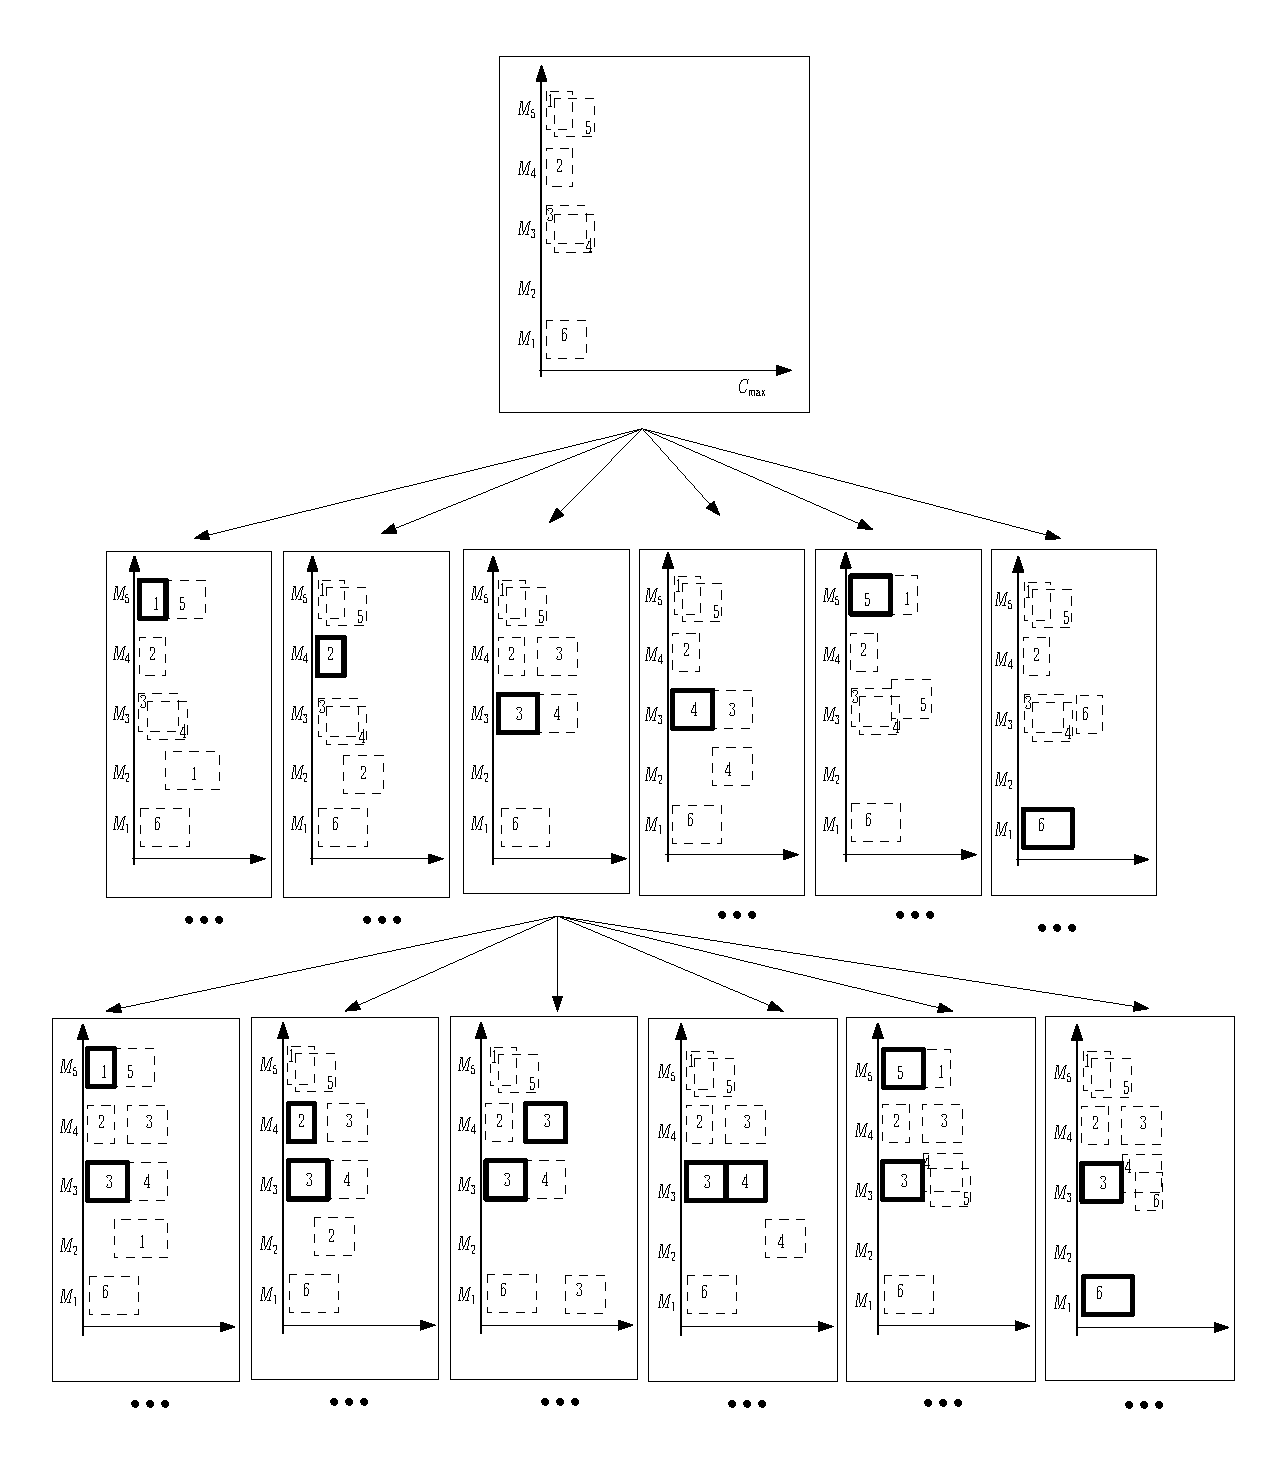
\includegraphics[width=\columnwidth]{gametree}
\caption[Partial Game Tree for JSP]{Partial Tree for job-shop scheduling problem for the first two dispatches. 
Top layer depicts all possible dispatches (dashed) for an empty schedule. 
Middle layer depicts all possible dispatches given that one of the dispatches from the layer above has been executed 
(solid). 
Bottom layer depicts when job $J_3$ on machine $M_4$ has been chosen to be dispatched from the previous layer, 
moreover it depicts all possible next dispatches from that scenario.}
\label{fig:jssp:gametree}
\end{figure}


However, one can easily see that this sequence of task assignments is by no means unique. Inspecting a partial 
schedule further along in the dispatching process such as in Fig.~\ref{fig:jssp:gametree} (top layer), then let's say 
$J_1$ 
would be dispatched next, and in the next iteration $J_2$. Now this sequence would yield the same schedule as if $J_2$ 
would have been dispatched first and then $J_1$ in the next iteration, i.e. these are non-conflicting jobs. Which 
indicates that some of the nodes in the tree can merge. In the meantime the state of the schedules are different and 
thus their features, although they manage to merge with the same (partial) schedule at a later date.  % ATHUGASEMD 1 
%-- SEQ. REP NON-UNIQUE
In this particular instance one can not infer that choosing $J_1$ is better and $J_2$ is worse (or vice versa) since they can both yield the same solution.

Furthermore, in some cases there can be multiple optimal solutions to the same problem instance. Hence not only is the 
sequence representation `flawed' in the sense that slight permutations on the sequence are in fact equivalent w.r.t. 
the end-result, but varying permutations on the dispatching sequence (given the same partial initial sequence) can 
result in very different complete schedules but the same makespan, and thus same deviation from optimality $\rho$ 
defined by~\eqref{eq:ratio}, which is the measure under consideration. Care must be taken in this case that neither 
resulting features are labelled as undesirable or suboptimal. Only the resulting features from a dispatch resulting in 
a suboptimal solution should be labelled undesirable. 

The creation of the tree for job-shop scheduling can be done recursively for all possible permutation of dispatches, 
in the manner described above, resulting in a full \mbox{$n$-ary} tree %(since $|\mathcal{R}|\leq n$)
of height $\ell=n\cdot m$. Such an exhaustive search would yield at the most $n^{\ell}$ leaf nodes (worst case scenario being that no sub-trees merge). Now, since the internal vertices, i.e. partial schedules, are only of interest to learn,\footnote{The root is the empty initial schedule and for the last dispatch there is only one option left to dispatch, so there is no preferred `choice' to learn.} the number of those can be at the most \mbox{${}^{n^{\ell}-1}/_{n-1}$}.
Even for small dimensions of $n$ and $m$ the number of internal vertices are quite substantial and thus 
computationally expensive to investigate them all. 
%Not to mention that this is done iteratively for all $N$ problem instances.



The optimum makespan is known for each problem instance. 
At each time step (i.e. layer of the tree) a number of feature pair are created, they consist of the features 
$\vphi_o$ resulting from optimal dispatches $o\in\mathcal{O}^{(k)}$, versus features $\vphi_s$ resulting from 
suboptimal dispatches $s\in\mathcal{S}^{(k)}$ at time $k$. Note, 
$\mathcal{O}^{(k)}\cup\mathcal{S}^{(k)}=\mathcal{R}^{(k)}$ and $\mathcal{O}^{(k)}\cap\mathcal{S}^{(k)}=\emptyset$.
In particular, each job is compared against another job of the ready-list, $\mathcal{R}^{(k)}$, and if the makespan differs, i.e. $C_{\max}^{(s)}\gneq C_{\max}^{(o)}$, an optimal/suboptimal pair is created, however if the makespan would be unaltered the pair is omitted since they give the same optimal makespan. This way, only features from a dispatch resulting in a suboptimal solution is labelled undesirable.

The approach taken here is to verify analytically, at each time step, by fixing the current temporal schedule as an initial state, whether it can indeed \emph{somehow} yield an optimal schedule by manipulating the remainder of the sequence. This also takes care of the scenario that having dispatched a job resulting in a different temporal makespan would have resulted in the same final makespan if another optimal dispatching sequence would have been chosen. That is to say the data generation takes into consideration when there are multiple optimal solutions to the same problem instance. 

\section{Selecting preference pairs}\label{sec:S:strategies}
At each dispatch iteration $k$ a number of preference pairs are created which can then be multiplied by the number of problem instance $N$ created. A separate data set is deliberately created for each dispatch iterations, as the initial feeling is that dispatch rules used in the beginning of the schedule building process may not necessarily be the same as in the middle or end of the schedule. As a result there are $\ell$ linear scheduling rules for solving a $n \times m$ job-shop, specified by a set of preference pairs for each step,  
\begin{equation}
S = \left\{\left\{\vphi_o-\vphi_s,+1\right\},\left\{\vphi_s-\vphi_o,-1\right\}
\;|\;\forall o\in \mathcal{O}^{(k)},s\in \mathcal{S}^{(k)}
\right\} \quad \forall k\in\{1,\ldots,\ell\}\label{eq:Sjssp}
\end{equation}
The reader is referred to~\cite{InRu11a} for a detailed description of how the linear ordinal regression model is trained on preference set $S$. Defining the size of the preference set as $l=\abs{S}$, if $l$ is too large, then re-sampling may be needed to be done in order for the ordinal regression to be computationally feasible. 


% % % I'm assuming that this was not done.! Nope. 
%Due to the nature of the sequence representation, the earlier stages of the dispatching are more or less equivalent 
%(and thus irrelevant), hence it is appropriate to follow some random optimal path to begin with and then follow some 
%(if not all possible) optimal paths until completion at step $\ell$. The strategy approached in  \cite{InRu11a} was 
%to 
%follow some optimal job $J_j\in\mathcal{O}^{(k)}$, thus creating 
%$\abs{\mathcal{O}^{(k)}}\cdot\abs{\mathcal{S}^{(k)}}$ 
%feature pairs at each dispatch $k$. %, resulting in a training size of,
%\begin{equation}\label{eq:sizeS_b}
%l =  \sum_{i=1}^N \left(2 \abs{\mathcal{O}^{(k)}_i}\cdot \abs{\mathcal{S}^{(k)}_i} \right)
%\end{equation}

\subsection{Trajectory sampling strategies}
The following trajectory sampling strategies were explored for adding preference pairs to $S$,
\begin{description}
\item[$S^{opt}$] at each dispatch some (random) optimal task is dispatched.
\item[$S^{cma}$] at each dispatch the task corresponding to highest priority, computed with fixed weights $\vec{w}$, which were obtained by optimising the mean for~\eqref{eq:ratio} with CMA-ES. 
\item[$S^{mwr}$] at each dispatch the task corresponding to most work remaining is dispatched, i.e. following the simple dispatching rule MWR.
\item[$S^{rnd}$] at each dispatch some random task is dispatched.
\end{description}
In the case of $S^{mwr}$ and $S^{cma}$ it is sufficient to explore each trajectory exactly once for each problem instance. Whereas, for $S^{opt}$ and $S^{rnd}$ there can be several trajectories worth exploring, however, only one is chosen (at random). 
It is noted that since the number of problem instances $N_{\text{train}}$ is large, it is deemed sufficient to explore one trajectory for each instance, in those cases as well.

\subsection{Ranking strategies}
The following ranking strategies were implemented for adding preference pairs to $S$,
\begin{description}
\item[$S_b$] all optimum rankings $r_1$ versus all possible sub-optimum rankings $r_i$, $i\in\{2,\ldots,n'\}$, preference pairs are added, i.e. same basic set-up as in~\cite{InRu11a}. %Note, $|S_b|$ is defined in~\eqref{eq:sizeS_b}.
\item[$S_f$] full subsequent rankings, i.e. all possible combinations of $r_i$ and $r_{i+1}$ for $i\in\{1,\ldots,n'\}$, preference pairs are added.
\item[$S_p$] partial subsequent rankings, i.e. sufficient set of combinations of $r_i$ and $r_{i+1}$ for $i\in\{1,\ldots,n'\}$, are added to the training set -- e.g. in the cases that there are more than one operation with the same ranking, only one of that rank is needed to compared to the subsequent rank. Note that $S_p\subset S_f$.
\end{description}
where $r_1>r_2>\ldots>r_{n'}$ ($n'\leq n$) are the rankings of the ready-list, $\mathcal{R}^{(k)}$, at time step $k$.

\section{Experimental study}\label{sec:expr:locallin}

To test the validity of different ranking and strategies from section~\ref{sec:S:strategies}, a training set of \mbox{$N_{\text{train}}=500$} and test set of $N_{\text{test}}=500$ problem instances of 6 jobs 5 machines job-shop are generated for the random and random-narrow problem space distributions. Where random and random-narrow are denoted $\mathcal{P}_{jrnd}$ and $\mathcal{P}_{jrndn}$ and processing times are drawn from a uniform distribution $\mathcal{U}(1,99)$ and $\mathcal{U}(45,55)$, respectively. Note that for both problem spaces considered there is a random $\sigma$ permutations of job orderings. 

The optimum makespan is denoted 
$C_{\max}^{\text{opt}}$, and the makespan obtained from the linear learning model by $C_{\max}^{\text{model}}$. Since 
the optimal makespan varies between problem instances the performance measure is the following, 
\begin{equation}\label{eq:ratio}\rho=\frac{C_{\max}^{\text{model}}-C_{\max}^{opt}}{C_{\max}^{\text{opt}}}\cdot 
100\%\end{equation}
which indicates the percentage relative deviation from optimality. 

The size of the preference set, $S$, for different trajectory and ranking strategies is depicted in Fig.~\ref{fig:sizeofprefset} for $\mathcal{P}_{jrnd}$ (above) and $\mathcal{P}_{jrndn}$ (below). 
The figure is divided vertically by problem space and horizontally by trajectory schemes.
 

A linear ordinal regression model (PREF) was created for each preference set, $S$, for problem spaces $\mathcal{P}_{jrnd}$ and $\mathcal{P}_{jrndn}$. A box-plot with the results of percentage relative deviation from optimality, $\rho$, defined by~\eqref{eq:ratio}, is presented in Fig.~\ref{fig:results}. The boxplots are grouped w.r.t. trajectory schemes and color-coded w.r.t. ranking schemes. 
Moreover, the simple priority dispatching rule MWR and the weights obtained by the CMA-ES optimisation used to obtain the preference sets $S^{mwr}$ and $S^{cma}$ respectively, are shown in black in the far left of the group for comparison.
From the figure it is apparent there can be a performance edge gained by implementing a particular ranking or trajectory strategy, moreover the behaviour is analogous across different disciplines. 
Main statistics are reported in Tables~\ref{tbl:results:jrnd} and~\ref{tbl:results:jrndn} for $\mathcal{P}_{jrnd}$ and $\mathcal{P}_{jrndn}$, respectively. Models are sorted w.r.t. mean relative error.

Note that $S_{a}$ denotes that all rankings were explored, i.e. $S_{a}=S_b\cup S_f\cup S_p$. Similarly, $S^{all}=S^{opt}\cup S^{cma}\cup S^{mwr} \cup S^{rnd}$ for all trajectories.


\begin{figure} \centering
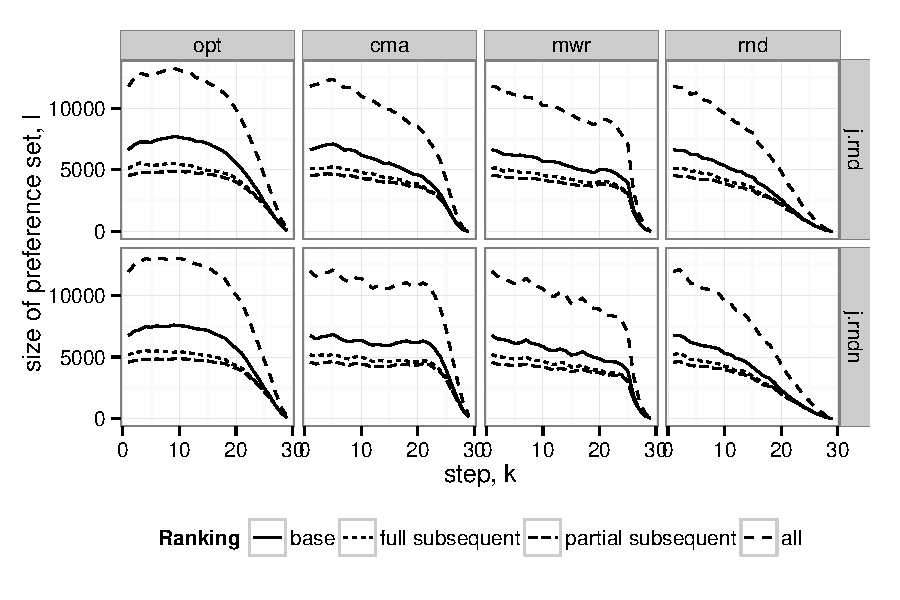
\includegraphics[width=\textwidth]{numTrainingData}
\caption{Size of preference set, $l$ for different trajectory and ranking strategies, given problem spaces $\mathcal{P}_{jrnd}$ (above) and $\mathcal{P}_{jrndn}$ (below).}
\label{fig:sizeofprefset}
\end{figure}


\begin{figure}\flushright \hfill
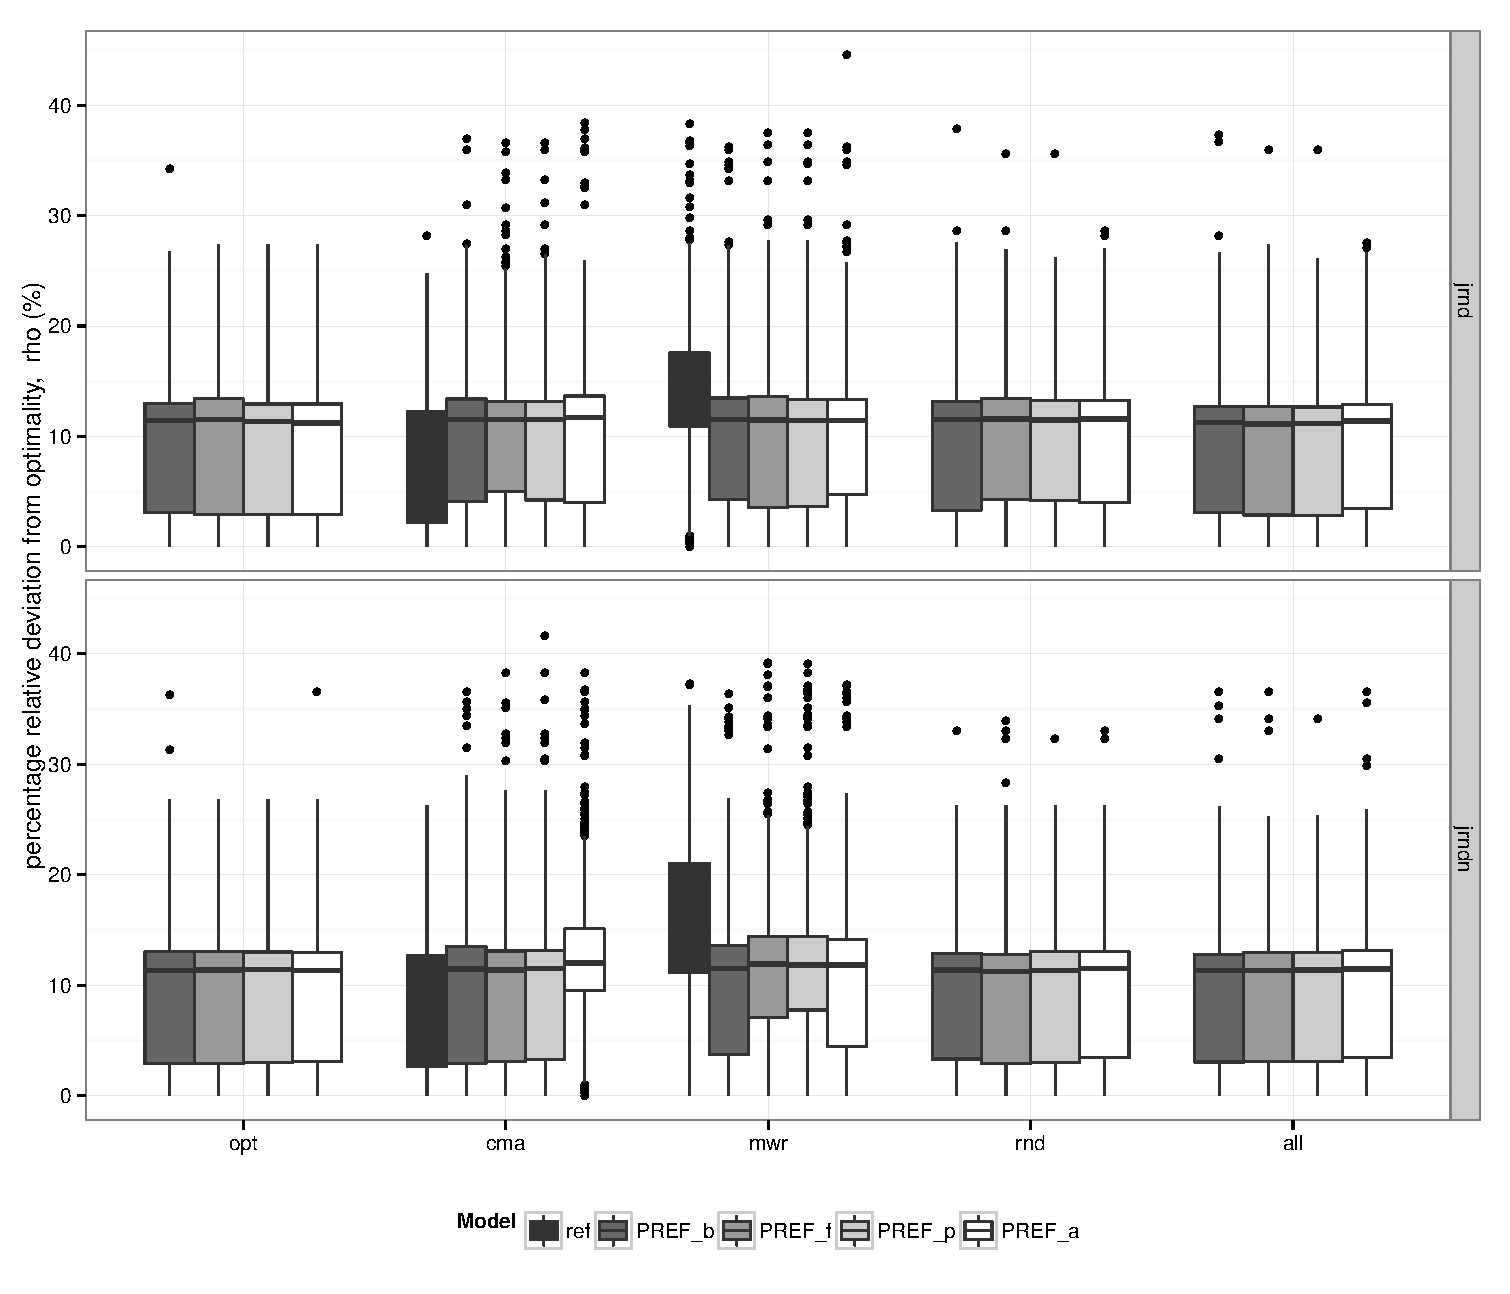
\includegraphics[width=\textwidth]{boxplot} 
\caption{Box-plot of results for linear ordinal regression model trained on various preference sets using test sets for problem spaces $\mathcal{P}_{jrnd}$ (above) and $\mathcal{P}_{jrndn}$ (below). Results are grouped by trajectories and color-coded w.r.t. ranking scheme. }
\label{fig:results}
\end{figure}
 
\input{tables/resultsjrnd.txt}
\input{tables/resultsjrndn.txt}
 
 

\subsection{Ranking strategies}
There is no statistical difference between $S_f$ and $S_p$ ranking-schemes across all trajectory disciplines (cf. 
Fig.~\ref{fig:results}), which is expected since $S_f$ is designed to contain 
the same preference information as $S_f$. The results hold for both problem spaces. 

Combining the ranking schemes, $S_{a}$, does not improve the individual ranking-schemes, across all  disciplines there is no statistical difference between $S_b$, $S_f$ nor $S_p$ and $S_{a}$, save $S_{cma}|\big|_{\mathcal{P}_{jrndn}}$ which yielded a considerably worse mean relative error. 

Moreover, there is no statistical difference between either of the Pareto ranking-schemes outperform and the original $S_b$ set-up from~\cite{InRu11a}. However overall, the Pareto-ranking schemes results in lower mean relative error not to mention that a smaller preference set is preferred, it is opted to use the $S_{p}$ ranking scheme. 

Moreover, it is noted that the learning algorithm is able to significantly outperform the original heuristics, MWR, used to create the training data $S^{mwr}$. The linear ordinal regression models based on $S^{mwr}$ are significantly better than MWR, irrespective of the ranking schemes. Whereas the fixed weights found via CMA-ES outperform the linear ordinal regression models for all ranking schemes. This implies that ranking scheme is relatively irrelevant. The results hold for both problem spaces. 


\subsection{Trajectory sampling strategies}
Learning preference pairs from a good scheduling policies, such as $S^{cma}$ and $S^{mwr}$, can give favourable results, however tracking optimal paths yields generally a mean relative error. 

It is particularly interesting there is no statistical difference between $S^{opt}$ and $S^{rnd}$ for both 
$\mathcal{P}_{jrnd}$ and $\mathcal{P}_{jrndn}$ ranking-schemes. That is to say, tracking optimal dispatches gives the same performance as completely random dispatches. This indicates that exploring 
only optimal trajectories can result in a training set where the learning algorithm is inept to determine good 
dispatches in the circumstances when newly encountered features have diverged from the learned feature set labelled to optimum solutions. 

Finally, $S^{all}$ and $S^{opt}$ gave the best combination for $\mathcal{P}_{jrnd}$ and $\mathcal{P}_{jrnd}$, however in the latter case $S^{rnd}$ had the best mean relative error although not statistically different from $S^{all}$ and $S^{opt}$. 

For $\mathcal{P}_{jrnd}$  the best mean relative error was for $S^{all}$, in that case adding random suboptimal trajectories with the optimal trajectories gave the learning algorithm a greater variety of preference pairs for getting out of local minima. Therefore a general trajectory scheme would to explore both optimal with suboptimal paths.

\subsection{Following CMA-ES guided trajectory}
The rational for using the $S^{cma}$ strategy was mostly due to the fact a linear classifier is creating the training data (using the weights found via CMA-ES optimisation), hence the training data created should be linearly separable, which in turn should boost the training accuracy for a linear classification learning model. However, this is not the case, since PREF$^{cma}$ does not improve the original CMA-ES heuristic which 
was used to guide its preference set $S^{cma}$. However the $S^{cma}$ approach is preferred to that of $S^{mwr}$, so there is some information gained by following the CMA-ES obtained weights instead of simple priority dispatching rules, such as MWR. 

%Let's inspect the CMA-ES guided training data more closely, in particular the linear weights for~\eqref{eq:jssp:linweights}. The weights are depicted in Fig.~\ref{fig:weights} for problem space $\mathcal{P}_{jrnd}$ (above) and $\mathcal{P}_{jrndn}$ (below). The original weights found via CMA-ES optimisation, that are used to guide the collection of training data, are depicted dotted whereas weights obtained by the linear classification model for $S_p^{cma}$ are depicted solid. 

%From the CMA-ES experiments it is clear that a lot of weight is applied to the $w_6$ that corresponds implementing MWR, yet the existing weights for other features converges the training data to a more ``better'' training set to learn. Arguably, the training set could be even better, however implementing CMA-ES is rather costly %

% NO LONGER THE CASE
%. It might also be an artefact due the fact the training set during the CMA-ES search is different to the data generation described in Sec.~\ref{sec:S:strategies} is completely different, hence the different scaling parameters for the features might influence the results. Moreover, the CMA-ES is minimising the makespan directly, whereas the supervised linear models are learning to discriminate optimal versus suboptimal features sets that implies a better deviation from optimality later on. 

%\begin{figure}\centering
%\includegraphics[width=\textwidth]{hi}
%\caption{Linear weights for problem spaces $\mathcal{P}_{jrnd}$ (above) and $\mathcal{P}_{jrndn}$ (below). Weights ($w_1$ to $w_{13}$ from left to right, top to bottom) found via CMA-ES optimisation (red), and weights found via learning classification model based on $S_p^{cma}$ (blue). }\label{fig:weights}
%\end{figure}

\subsection{Summary and conclusion}
As the experimental results illustrate in section~\ref{sec:expr:locallin}, the classification of optimal\footnote{Here the tasks labelled `optimal' do not necessarily yield the optimum makespan (except in the case of following optimal trajectories), instead these are the optimal dispatches for the given partial schedule.} and suboptimal features are of paramount importance. The subsequent rankings are not of much value, since they are disregarded anyway. However, the trajectories to create training instances have to be varied.

Unlike~\cite{Siggi10,Malik08,Russell09} learning only on optimal training data was not fruitful. However, inspired by the original work by~\cite{Siggi05}, having heuristic guide the generation of training data, but with nevertheless optimal labelling based on a solver, gave meaningful preference pairs which the learning algorithm could learn. In conclusion, henceforth, the training data will be generated with $S_{p}^{all}$ scheme for the authors' future work.

Based on these preliminary experiments, we continue to test on a greater variety of problem data distributions for scheduling, namely job-shop and permutation flow-shop problems. Once training data has been carefully created, global dispatching rules can finally be learned, with the hope of implementing them for a greater number of jobs and machines. This is the focus of our current work.


%\begin{acknowledgements}
%Put any acknowledgements here, or delete this section
%\end{acknowledgements}

% BibTeX users please use one of
%\bibliographystyle{spbasic}      % basic style, author-year citations
\bibliographystyle{spmpsci}      % mathematics and physical sciences
%\bibliographystyle{spphys}       % APS-like style for physics
\bibliography{references} % name your BibTeX data base

\end{document}
% end of file sample.tex

